\chapter{Stability of fixed points}
Now we would like to begin to explore the behaviour of dynamical systems around fixed points. This will allow us to find out if we should expect to observe a fixed state, and to understand what happens if we perturb the system away from this fixed state.
\section{Basic definitions}
Consider
\begin{align}
	\dot{ {x}}=f( {x},t),\  {x} \in \mathbb{R}^{n},\ f\in C^{1}.
\end{align}
Assume that $ {x}=0$ is a fixed point, i.e. $f({0},t) = {0}$ for all $t \in \mathbb{R}$. If the fixed point is originally at ${x}_0\neq {0}$, shift it to zero by letting $\tilde{ {x}}:= {x}- {x}_0$, therefore 
\begin{align}
	\dot{\tilde{ {x}}} = \dot{ {x}} = f( {x}_0 + \tilde{ {x}}, t) = \tilde{f}(\tilde{ {x}}, t).
\end{align}
We would like to understand how the dynamical system behaves near its equilibrium state. To this end we introduce the following definitions.
\begin{definition}[Lyapupnov Stability]
	$ {x}={0}$ is stable if for all $t_0$, for all $\epsilon>0$ small enough, there exists a $\delta=\delta(t_0, \epsilon)$, such that for all $ {x}_0 \in \mathbb{R}^{n}$ with $\| {x}_0\| \leq \delta$, we have 
	\begin{align}
		\left \|  {x}(t;t_0,  {x}_0) \right\| \leq \epsilon \quad \forall t \geq t_0.
	\end{align}
\begin{figure}[h!]
	\centering
	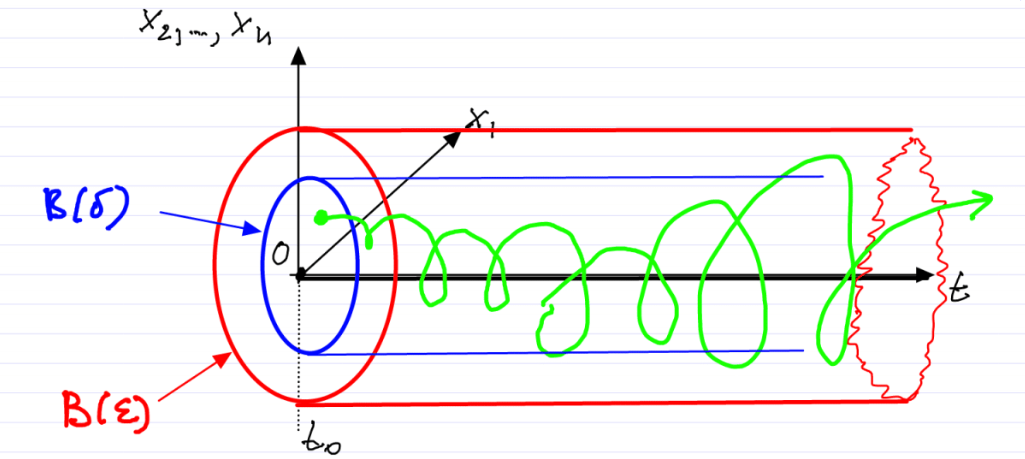
\includegraphics[width=0.7\textwidth]{figures/ch2/1lyapunov_stability.png}
	\caption{An example such a $\delta$, $B(r)$ represents the $n$-dimensional ball of radius $r$.}
	\label{fig:lyapunov_stability_def}
\end{figure}
\end{definition}

\begin{ex}[Stability of lower  equilibrium of the pendulum]
	Recall the equation of motion of the pendulum $\ddot{\varphi} + \sin(\varphi) = 0$, that we transform into a first order ODE by setting $x_1 = \varphi$ and $x_2 = \dot{\varphi}$ to obtain
	\begin{align}
		\begin{dcases}
		\dot{x}_1 = x_2 \\
	\dot{x}_2 = -\sin(x_1).
		\end{dcases}
	\end{align}
	For small $\epsilon>0$, this geometric procedure gives a $\delta(\epsilon)>0$ such that the definition of stability is satisfied for $ {x}=0$. We can see in Fig. \ref{fig:pend_lower_stability}  that for any point chosen within the blue circle, it's trajectory remains within the red circle for all time (cf. Fig. \ref{fig:lyapunov_stability_def}. Therefore $ {x}=0$ is (Lyapunov) stable.
	\begin{figure}[h!]
		\centering
		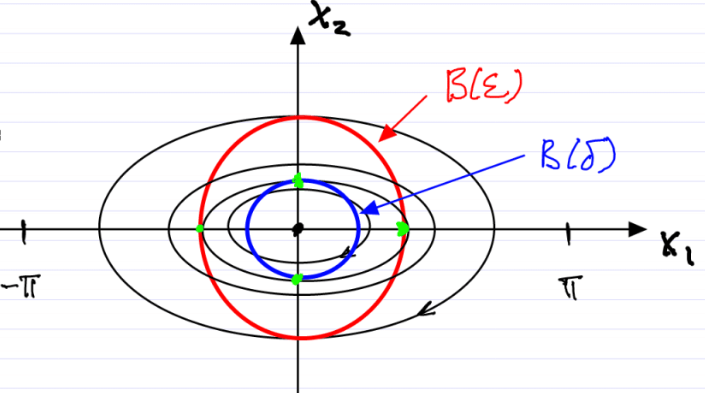
\includegraphics[width=0.5\textwidth]{figures/ch2/2pendulum_stability.png}
		\caption{Stability of lower equilibrium for the pendulum, here $0<\epsilon<\pi $.}
	\label{fig:pend_lower_stability}
	\end{figure}
\end{ex}

\begin{definition}[Asymptotic stability]
	The fixed point $ {x}=0$ is \emph{asymptotically stable} if
\begin{enumerate}
	\item it is stable,
	\item for all $t_0$, there exists $\delta_0(t_0)$ such that for every $ {x}_0$ with $\|  {x}_0 \| \leq \delta_0$ we have
		\begin{align}
			\boxed{\lim_{t\to \infty }  {x}(t; t_0,  {x}_0) = 0.}
		\end{align}
\end{enumerate}
\begin{figure}[h!]
	\centering
	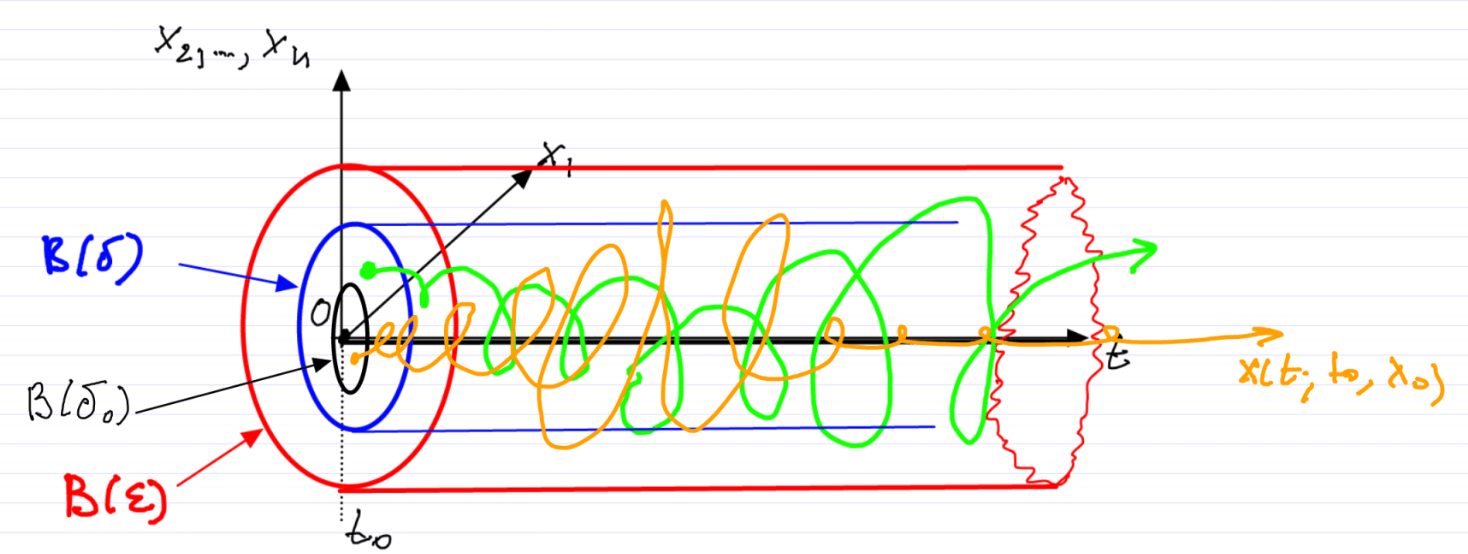
\includegraphics[width=0.7\textwidth]{figures/ch2/3asymp_stability.png}
	\caption{An example for an asymptotically stable fixed point (black trajectory).}
\end{figure}
\end{definition}

\begin{definition}[Domain of attraction] 
	The \emph{domain of attraction} is the set of all $ {x}_0$'s for which
	\begin{align}
		\boxed{\lim_{t\to \infty } {x}(t;t_0,  {x}_0)=0. }	
	\end{align}
	
\end{definition}

\begin{ex}[Damped pendulum]
	We have the equation of motion with the linear damping coefficient $c$
	\begin{align}
		\ddot{\varphi} + c \dot{\varphi} + \sin(\varphi) = 0,\quad c>0.
	\end{align}
	Transforming into a first-order ODE with $x_1 = \varphi$ and $x_2 = \dot{\varphi}$ gives
	 \begin{align}
		\begin{dcases}
		\dot{x}_1 = x_2\\ \dot{x}_2 = -cx_2 - \sin(x_1).
		\end{dcases}
	\end{align}
The total energy is given by
\begin{align}
	E = \frac{1}{2}x_2^2 + \left( 1 - \cos(x_1) \right). 
\end{align}
Further we have the rate of energy change
\begin{align}
\frac{d}{dt} E(x_1(t), x_2(t)) = x_2 \left(\dot{x}_2 + \sin(x_1) \right) = -c x_2^{2}.
\end{align}
\begin{figure}[h!]
	\centering
	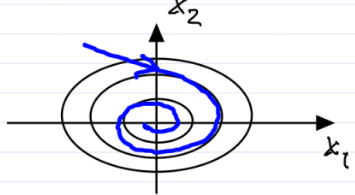
\includegraphics[width=0.35\textwidth]{figures/ch2/4damped_pendulum.png}
\end{figure}

Therefore, along trajectories energy decreases monotonically. By the $C^0$ dependence of the trajectory on initial conditions, the trajectories remain close to the undamped oscillations for small $c>0$. We conclude that trajectories are inward spirals for a small dissapation $c>0$ small. The fixed point $ {x}=0$ is still Lyapunov stable, but asymptotic stability does not yet follow (is the limit of $ {x}(t)$ equal to 0?).
\begin{remark}[LaSalle's invariance principle]
	This conclusion follows rigorously from LaSalle's invariance principle, namely if we assume that $\dot{ {x}}=f( {x})$, $f \in C^1$, and that there exists a $V\in C^1$ with 
	\begin{align}
		\dot{V} = \frac{dV( {x}(t))}{dt} \leq 0.	
	\end{align}
	Then the set of accumulation points for any trajectory is contained in the set of trajectories that stay within the set $I=\{ {x} \in \mathbb{R}^{n}:\ \dot{V}( {x}) = 0\}$.
\end{remark}
\end{ex}

\begin{ex}[]
	Consider the following dynamical system in polar coordinates, i.e. $r\cos(\theta) = x$ and $r \sin(\theta) = y$,
	\begin{align}
		\begin{dcases}
			\dot{r} = r(1-r) \\ \dot{\theta} = \sin^2\left( \frac{\theta}{2} \right).
		\end{dcases}
	\end{align}
	Note that $r=0$ is a fixed point, the set $r=1$ is an invariant circle, and the set $\theta=0$ is an invariant set. An invariant set is a set such that if the dynamical system is started on the set, it remains in the set for all time. Examining the radial evolution reveals that the equation of motion decouples. We see that $\dot{\theta}\geq 0$, so rotation is either positive or null.
	\begin{figure}[h!]
		\centering
		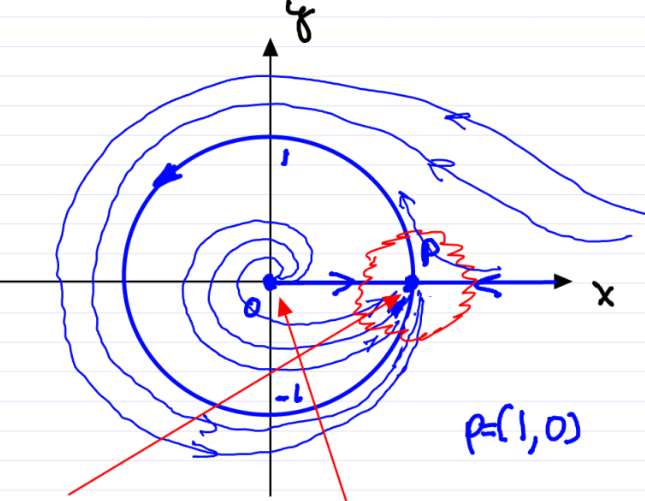
\includegraphics[width=0.5\textwidth]{figures/ch2/5polar_cds.png}
		\caption{Phase portrait of the dynamical system in cartesian coordinates, with the red arrows pointing to the two unstable equilibria.}
		\label{fig:polar_attractor}
	\end{figure}

	However, inspecting Fig. \ref{fig:polar_attractor} we see that that $p=(1,0)$ is an example of an attractor: a set with an open neighborhood of points that all approach the set as $t\to \infty $. From Fig. \ref{fig:polar_attractor} we can also see that both of the fixed points, $(0,0)$ and $(1,0)$, are not stable.
\end{ex}

\begin{definition}[Invariant set]
	The set $S \subset P$ is an \emph{invariant set} for the flow map $F^{t}:P \to P$ if $F^{t}(S) =S$ for all $t \in \mathbb{R}$.
\end{definition}

\begin{definition}[Unstable point]
	A fixed point $ {x}=0$ is unstable if it is not stable.
\end{definition}

\begin{remark}[]
	We can negate a mathematical statement by using the reverse relational operators outside the statements involving these operators i.e. $ \exists \to \forall $ and $\forall \to \exists $. For example we have for continuity $\forall \epsilon\ \exists \delta:\  \|f( {x}) - f( {y}) \| < \epsilon$ if $ \| {x}- {y} \|<\delta$, meanwhile for discontinuity we have  $\exists \epsilon:\ \forall \delta:\  \|f( {x}) - f( {y}) \| \geq  \epsilon$ for $ \| {x}- {y} \|< \delta$.

	In our case for stability we have
	\begin{align}
		\forall \epsilon,t_0: \quad \exists \delta>0: \quad \forall  {x}_0  \textrm{ with }  \| {x}_0 \| < \delta: \quad  \| {x}(t) \|\leq \epsilon \quad \forall t\geq t_0.
	\end{align}
Meanwhile for instability 
\begin{align}
	\exists \epsilon,t_0:\quad \underbrace{\forall \delta>0}_{ \textrm{``for arbitrarily small"} }:\quad \exists  {x}_0  \textrm{ with }  \| {x}_0 \|<\delta: \quad  \| {x}(t) \|>\epsilon \quad \underbrace{\exists t\geq t_0}_{ \textrm{``for some"} }.
\end{align}
This negation is demonstration in Fig. \ref{fig:instable_def}.
\begin{figure}[h!]
	\centering
	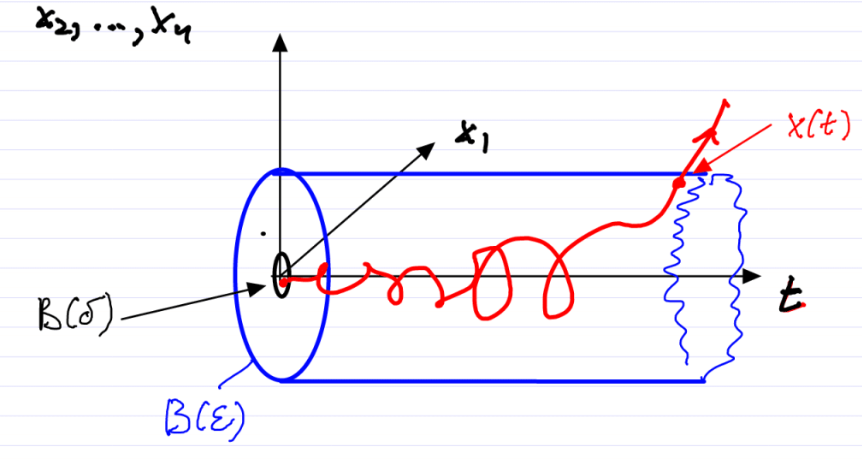
\includegraphics[width=0.5\textwidth]{figures/ch2/6unstable_def.png}
	\caption{Example of an unstable fixed point, with the red trajectory representing a trajectory starting arbitraritly close to the fixed point, leaving a given $\epsilon$-ball.}
	\label{fig:instable_def}
\end{figure}
\end{remark}

\begin{remark}[]
	By $C^0$ dependence of trajectories on initial conditions, if $ {x}(t;t_0, {x}_0)$ leaves $B(\epsilon)$, then for $\tilde{ {x}}_0$ close enough to $ {x}_0$, $ {x}(t;t_0,\tilde{ {x}}_0)$ also leaves $B(\epsilon)$. Since this is true on an open set around ${x}_0$, the measure of such trajectories in nonzero, the instability is observable!
\end{remark}

\begin{ex}[Unstable fixed point of pendulum]
	In contrast, we can have that infinitely many trajectories converge to the fixed point, yet it is still unstable, as illustrated in Fig. \ref{fig:convergent_unstable}. In fact, the converging trajectories form a measure-zero set, thus the stability near the unstable equilibrium is unobservable.
	\begin{figure}[h!]
		\centering
		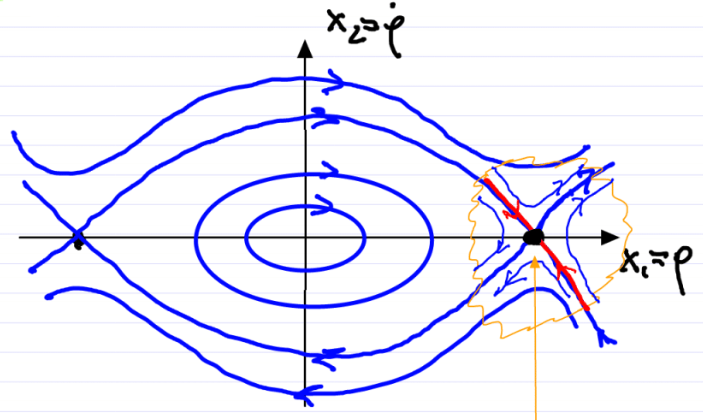
\includegraphics[width=0.6\textwidth]{figures/ch2/7unstable_pendulum.png}
		\caption{The phase portrait around the unstable fixed point of the pendulum, with the stable trajectories (red).}
		\label{fig:convergent_unstable}
	\end{figure}
	
\end{ex}
\newpage
\section{Stability based on linearization}
We would like to derive a more general method to analyze the stability of fixed points, thus we try to simplify our system around the fixed point and discover what this can tell us about the full (unsimplified) system. In the following section we shall always assume that our system is autonomous. We will have the following setup
\begin{align*}
	\dot{ {x}}=f( {x}),\quad f\in C^1,\quad  {x}=
	\begin{pmatrix}
		x_1\\ \vdots \\ x_n
	\end{pmatrix}\in \mathbb{R}^{n}, \quad 
	{p} = 
\begin{pmatrix}
	p_1 \\ \vdots \\ p_n 
\end{pmatrix}
\in \mathbb{R}^{n}. \numberthis \label{eq:star}
\end{align*}

If $f({p} )={0} $, then ${p} $ is a fixed point. By transforming using ${y} = {x} - {p} $, we have that in the transformed system ${y} = {0} $ is a fixed point. Furthermore, we have that around ${y} = {0} $ the ODE is 
\begin{align}
	\dot{{y} } = f({p} + {y} ) = \underbrace{f({p} )}_{=0} + Df({p} ){y} + \mathcal{O}(\| {y} \|^2) = Df({p} ){y} + \mathcal{O}(\| {y} \|^2).
\end{align}
\begin{definition}[Linearized ODE]
	We define the \emph{linearization} of \eqref{eq:star} at the fixed point ${p} $ as 
	\begin{align*}
		\boxed{
		\dot{{y} } = {A} {y}; \quad {y} \in \mathbb{R}^{n},\quad {A} := Df({p} ) \in \mathbb{R}_{n \times n};\quad  Df(p) = 
	\left. \begin{pmatrix}
		\frac{\partial f_1}{\partial x_1} & \ldots & \frac{\partial f_1}{\partial x_n} \\
		\vdots & & \vdots \\
		\frac{\partial f_n}{\partial x_1} & \ldots & \frac{\partial f_n}{\partial x_n}
\end{pmatrix}\right|_{{x} = {p} }.} \numberthis \label{eq:sstar}
	\end{align*}
\end{definition}
Now we would like to study the stability of the fixed point ${y} =0$ in \eqref{eq:sstar}. From this analysis, we want to know the relevance of our results for the full nonlinear system \eqref{eq:star}.

\section{Review of linear dynamical systems}
Recall the setup
\begin{align}
	\dot{{y} } = {A} (t){y}, \quad {y} \in \mathbb{R}^{n}, \quad {A} \in \mathbb{R}^{n \times n}, \quad {A} \in C^{0}_{t}.
\end{align}
The following facts have already been established
\begin{itemize}
	\item We know that the global existence and uniqueness of solutions is guaranteed. 
	\item The superposition principle holds; namely the linear combination of solutions is also a solution.
	\item There exists a set of $n$ linearly independent solutions: $\varphi_1(t), \ldots, \varphi_n(t) \in \mathbb{R}_{n}$.
	\item The general solution is
		\begin{align}
			y(t) = \sum_{i=1}^{n} c_i \varphi(t) =
			\underbrace{\begin{bmatrix}
				\varphi_1(t) & \ldots & \varphi_n(t)
		\end{bmatrix}}_{\Psi(t):  \textrm{ fundamental matrix solution} }
		\underbrace{\begin{bmatrix}
			c_1 \\ \vdots \\ c_n
	\end{bmatrix}}_{c}
	= \Psi(t) {c}; \quad \dot{\Psi} = A(t) \Psi.			
		\end{align}
	\item We have the initial value problem ${y} (t_0) = {y} _0$ which implies
		\begin{align}
			\Psi(t_0) {c} = {y} _0 \implies {y} (t) = \underbrace{\Psi(t) \left[\Psi(t_0)\right]^{-1}}_{\phi(t):= F_{t_0}^{t}}{y} _0 
		\end{align}
		Where we used that the $\varphi_i(t)$ are linearly independent in the last equality. And we have the \emph{normalized fundamental matrix} $\phi(t)$ equal to the flow map, with $\phi(t_0)={I} $.
	\item In the autonomous case $\dot{{x} }= {A} {x} $ solutions can be practically constructed.
	\begin{enumerate} 
		\item \textbf{Explicit Solution} 
		\begin{align}
			\phi(t) = e^{{A} t} := \sum_{j=0}^{\infty } \frac{1}{j!} ({A} t)^{j}
		\end{align}
	With $0! =1$ and ${0} ^{0}= {I} $. We can verify that this is indeed a solution
	\begin{align}
		\dot{\phi}(t) = \sum_{j=1}^{\infty } \frac{1}{(j-1)!} ({A} t)^{j-1}{A} = {A} \sum_{j=0}^{\infty } \frac{1}{j!} ({A} t)^{j} = {A}  e^{{A} t} = {A} \phi(t).
	\end{align}
	Where we used that ${A} $ commutes with its powers in the second equality. We now have that each column of $\phi(t)$ satisfies $\dot{{y} } = {A} {y} $.	
	\begin{remark}[]
		For a scalar ODE $\dot{y}= a(t)y$ for $y \in \mathbb{R}$, the solution is known $y(t) = e^{\int_{t_0}^{t} a(s)ds}y_0$. However, this does not extend to the higher dimensional $\dot{{y} }= {A} (t){y} $. In fact, in general, $\phi(t) = e^{\int_{t_0}^{t} {A} (s)ds}$ is \underline{not} a solution. We can check this
	\begin{align}
		\dot{\phi} = \sum_{j=0}^{\infty } \frac{1}{j!} \frac{d}{dt} \left( \int_{t_0}^{t} {A} (s) ds \right)^{j} = \sum_{j=1}^{\infty } \frac{1}{(j-1)!} \left( \int_{t_0}^{t} {A} (s)ds \right)^{j-1} {A} (t) \neq {A} (t) \phi(t).
	\end{align}
	The nonequality holds as ${A} (t)$ does not generally commute with $\int_{}^{} {A} (s)ds$.
	\end{remark}

\item \textbf{Solution from eigenfunctions} If we have an autonomous system, we can solve the ODE without an infinite series. We have 
	\begin{align*}
		\dot{{y} } = {A} {y} ,\quad {y} \in \mathbb{R}^{n}, \quad {y} (0) = {y}_0. \numberthis \label{eq:onestar}
	\end{align*}
	Substituting $\varphi(t)=e^{\lambda t}{s} $ for $\lambda\in \mathbb{C}$ and ${s} \in \mathbb{C}^{n}$ into \eqref{eq:onestar} yields
\begin{align*}
	\lambda {s} = {A} {s} \implies ( {A} - \lambda {I} ) {s} = 0 \iff \det( {A} - \lambda {I} ) = 0 \numberthis \label{eq:twostar}.
\end{align*}
Therefore $\lambda$ must be an eigenvalue of ${A}$ and ${s} $ must be the corresponding eigenvector. We call $\det({A} - \lambda {I} )$ the \emph{characteristic equation} of ${A} $. Let $\lambda_1, \ldots , \lambda_n$ be the eigenvalues and ${s} _1, \ldots, {s} _n$ be the corresponding eigenvectors. In the case that some eigenvalues are repeated, some of the ${s} _i$ may be generalized eigenvectors. We then have two cases.
\begin{enumerate}
	\item ${A} $ is semisimple, i.e. the eigenvectors are linearly independent (which is always the case if the $\lambda_i$ all have algebraic multiplicity of one). Then we have the solution
		\begin{align}
			{y} (t) = \sum_{i=1}^{n} c_i e^{\lambda_i t}{s} _i = \sum_{j=1}^{n} c_j e^{ (\textrm{Re} \lambda_j) t} e^{i( \textrm{Im} \lambda_j)t} {s} _j.
		\end{align}
	Where we used $\lambda_j =  \textrm{Re} \lambda_j + i  \textrm{Im} \lambda_j$.	
\item ${A} $ is \underline{not} semisimple, i.e. has repeated eigenvalues (but not enough linearly independent eigenvectors). Then we assume that $\lambda_k$ has algebraic multiplicity $a_k > g_k$, where $a_k$ measures the multiplicity of $\lambda_k$ as a root of $\det({A} - \lambda {I} )=0$, and $g_k$ is the number of linearly independent eigenvectors for $\lambda_k$, also called the \emph{geometric muliplicity} of $\lambda_k$. Even in this case, $\lambda _k$ gives rise to $a_k$ linearly independent solutions of the form
	\begin{align}
		\underbrace{{P} _0}_{={s_k} } e^{\lambda _k t},\ {P} _1(t) e^{\lambda _k t}, \ {P}_2(t)e^{\lambda _k t}, \ldots, {P} _{a_{k-1}}(t)e^{\lambda _k t}
	\end{align}
	where ${P} _{j}(t)$ is a vector polynomial of $t$ of order $j$ or less.	
\end{enumerate}

	\end{enumerate}
\end{itemize}

\section{Stability of fixed points in autonomous linear systems}
First we note that we can bound our solution
\begin{align*}
	\| {y} (t) \| = \| \phi(t) {y} _0 \| \leq \underbrace{\| \phi(t) \|}_{ \textrm{Operator norm} } \| {y}_0 \| \leq C e^{\mu t} \| {y} _0 \|. \numberthis \label{eq:1star}
\end{align*}
Where $\mu = \max_j ( \textrm{Re} \lambda_j) + \nu $, with $\nu >0$, as small as needed, provided we increase $C$ appropriately. If ${A} $ is semisimple, then $\nu =0$ can be selected.
\begin{theorem}[Stability of fixed points in linear systems] \label{thm:lin_stab_eigv}
	Given ${y} =0$ a fixed point of the linear system $\dot{{y} } = {A} {y} $ with ${A} \in \mathbb{R}^{n \times n}$ the following statements hold:
	\begin{enumerate}
		\item Assume that $ \textrm{Re} \lambda _j < 0$ for all $j$. Then ${y} =0$ is asymptotically stable.
		\item Assume that $ \textrm{Re} \lambda _j \leq 0$ for all $j$, and for all $\lambda_k$ with $ \textrm{Re} \lambda_k = 0$ we have $a_k = g_k$. then ${y} =0$ is stable.
		\item Assume there exists a $k$ such that $ \textrm{Re} \lambda _k >0$. Then ${y} =0$ is unstable.
	\end{enumerate}
	These scenarios are illustrated in Fig. \ref{fig:eigv_setup}.
\end{theorem}
\begin{proof}
	\begin{enumerate}
		\item Pick $\epsilon > 0$, and select $\nu > 0$ small, such that $\mu <0$. Then pick $C> 0$ such that \eqref{eq:1star} holds, and let $\delta = \frac{\epsilon}{C}$. This implies (since $\| {y} _0\| \leq \delta $) that
			\begin{align}
				\| {y} (t) \| \leq \epsilon e^{\mu t} \leq \epsilon,
			\end{align}
		and
		\begin{align}
			\| {y} (t) \| \leq \epsilon e^{\mu t} \xrightarrow{t \to \infty } 0. 
		\end{align}
	Where the limit holds as $\mu < 0$.	
\item Again choose $\delta = \frac{\epsilon}{C}$ and note that $\mu  = \max_{j} ( \textrm{Re} \lambda _j) + \nu = 0 + \nu =0$ ($\nu =0$ as $a_k = g_k$). Then stability follows by \eqref{eq:1star}. However, asymptotic stability does not hold, as $\varphi(t) = C e^{i ( \textrm{Im} \lambda _j)t} $ solutions exist.

\item There exists a solution of the form
	\begin{align}
		{	\varphi}(t) = C_k e^{\lambda _k t} {s} _k = C_k e^{( \textrm{Re}  \lambda _k)t} e ^{i ( \textrm{Im} \lambda _k)t}{s} _k.
	\end{align}
In turn this implies
\begin{align}
	\| {\varphi}(t) \| = C_k e^{( \textrm{Re} \lambda_k) t} \| {s} _k \| \xrightarrow{t \to \infty} \infty .
\end{align}

	\end{enumerate}
\end{proof}
\begin{figure}[h!]
	\centering
	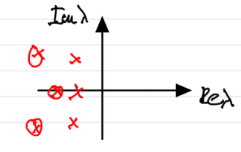
\includegraphics[width=0.3\textwidth]{figures/ch2/8eigv_setup1.png}
	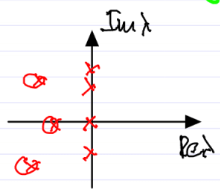
\includegraphics[width=0.3\textwidth]{figures/ch2/9eigv_setup2.png}
	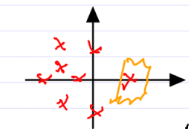
\includegraphics[width=0.3\textwidth]{figures/ch2/10eigv_setup3.png}
	\caption{Eigenvalue arrangements for scenarios (i), (ii), and (iii) (from left to right) in Theorem \ref{thm:lin_stab_eigv}}
	\label{fig:eigv_setup}
\end{figure}

\begin{ex}[Stability analysis of 2 degrees of freedom coupled oscillators]
	Given a rectangular mass $m$ with a spring of stiffness coefficient $k$ attached to each side extending to fixed walls in each cardinal direction. We want to know the stability of the equilibrium where all of the springs are equally extended. This dynamical system is depicted in Fig. \ref{fig:quad_spring}.
\begin{figure}[h!]
	\centering
	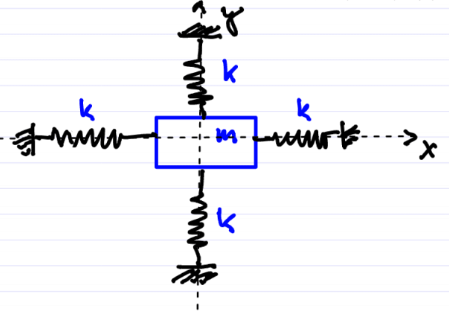
\includegraphics[width= 0.3\textwidth]{figures/ch2/11quad_spring.png}
\caption{Arrangement of coupled oscillators with rectangular mass in the middle.} \label{fig:quad_spring}
\end{figure}
First, note that this is a conservative system, i.e. $E=$ const. Next we transform the coordinates so that the equations of motion can be brought into the form of an ODE for this dynamical system
\begin{align}
	{x} = 
	\begin{pmatrix}
		x \\ \dot{x} \\ y  \\ \dot{y}
	\end{pmatrix}.
\end{align}
Thus we have a 4-dimensional, nonlinear, system of ODEs. We now linearize this at the fixed point $(x,y)= (0,0)$, i.e. $\dot{{x}} = {A} {x} $ with ${x} \in \mathbb{R}^{n}$.

The system exhibits full spatial symmetry in $x$ and $y$, hence the eigenmodes will be the same in the $x$ and $y$ directions. This means we have repeated, purely imaginary, pairs of eigenvalues for ${A} $:  $\lambda_{1,2}=\lambda_{3,4}= \pm i \omega $. It is clear that scenarios (i) and (iii) of Theorem \ref{thm:lin_stab_eigv} do not apply to the linearized ODE. So we need to check if (ii) applies.

We have that $ \textrm{Re} \lambda _{k}=0$ for $k=1,2,3,4$. Also $a_k=2$ for $k=1,2,3,4$. Now assume $g_k < 2$. Then there would exists solutions of the form $te^{\pm i \omega t}{s}_k$, but this would contradict the conservation of energy, as either the (nonnegative) kinetic energy and/or the (nonnegative) potential energy would grow unbounded. Hence, the total energy could not be conserved. Therefore we know that $g_k = a_k$ and we can apply (ii) to find $x=y=0$ is Lyapunov stable for the linearized system. What does this imply for the nonlinear system?
\end{ex}

\section{Stability of fixed points in nonlinear systems}
Following the previous example, we would like to know what information about the stability of fixed points of nonlinear systems we can derive from the linearized system. The full nonlinear system is
\begin{align*}
	\dot{{x} } = f(x),\quad f({x} _{0}) = {0}, \quad {x} \in \mathbb{R}^{n}, \quad f \in C^{1}. \numberthis \label{eq:unostar}
\end{align*}
And its linearization at the fixed point ${x} _0$ 
\begin{align*}
	\dot{{y} } = Df({x} _0){y}, \quad y\in \mathbb{R}^{n},\quad Df({x} _0) \in \mathbb{R}^{n\times n}
	\numberthis \label{eq:dosstar}.
\end{align*}
We would like to conclude that the linearized dynamics are qualitatively similar to the nonlinear dynamics. In order to study if this is the case, we have to formalize 'similar' mathematically.

\begin{definition}[$C^k$ equivalence of dyanimical systems]
Consider two autonomous dynamical systems:
\begin{enumerate}
	\item
		\begin{align*}
			\dot{{x} }=f({x}),\quad {x} \in \mathbb{R}^{n}, \quad f \in C^{1};\quad F^{t}: {x_0} \mapsto {x} (t;{x} _0). \numberthis \label{eq:uno}
		\end{align*} 
	\item	
		\begin{align}
			\dot{{x} }=g({x}),\quad {x} \in \mathbb{R}^{n}, \quad g \in C^{1};\quad G^{t}: {x_0} \mapsto {x} (t;{x} _0).
		\end{align}
\end{enumerate}
The two dynamical systems are \emph{$C^k$ equivalent}, for $k \in \mathbb{N}$, on an open set $U \subset \mathbb{R}^{n}$, if there exists a $C^k$ diffeomorphism $h: U \to U$ that maps orbits of (i) into orbits of (ii), while preserving the orientation but not necessarily the exact parameterization of the orbit by time. Specifically for all $x\in U$, any $t _1 \in \mathbb{R}$  there exists a $t_2 \in \mathbb{R}$ such that
\begin{align}
	\boxed{
		h(F^{t_1}({x})) = G^{t_2}(h(x)).
	}
\end{align}
$h:U\to U$ does this for all $x\in U$ in a $C^{k}$ fashion. This equivalence through a function $h$ is demonstrated in Fig \ref{fig:ck_equiv}.
\begin{figure}[h!]
	\centering
	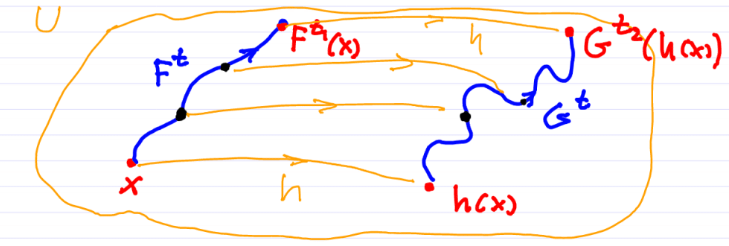
\includegraphics[width=0.7\textwidth]{figures/ch2/12ck_equiv.png}
	\caption{The function $h$ mapping the orbits of the dynamical system describing $F$ into the system describing $G$.}
	\label{fig:ck_equiv}
\end{figure}
\end{definition}

\begin{definition}[Topological equivalence]
	For $k=0$, $C^{k}$ equivalence is also called \emph{topological equivalence}. In this case, a continuous, invertible, deformation takes orbits of one system into the orbits of the other. Under these conditions,  $h:U\to U$ is called a \emph{homeomorhpism}.
\end{definition}
\begin{ex}[Topologically equivalent linear systems for $n=2$]
	To illustrate the meaning of topological equivalence, Fig. \ref{fig:topo_equiv} shows three linear systems ($\dot{{x} } = {Ax}  $ for $x\in \mathbb{R}^2$) which are topologically equivalent.
	\begin{figure}[h!]
		\centering
		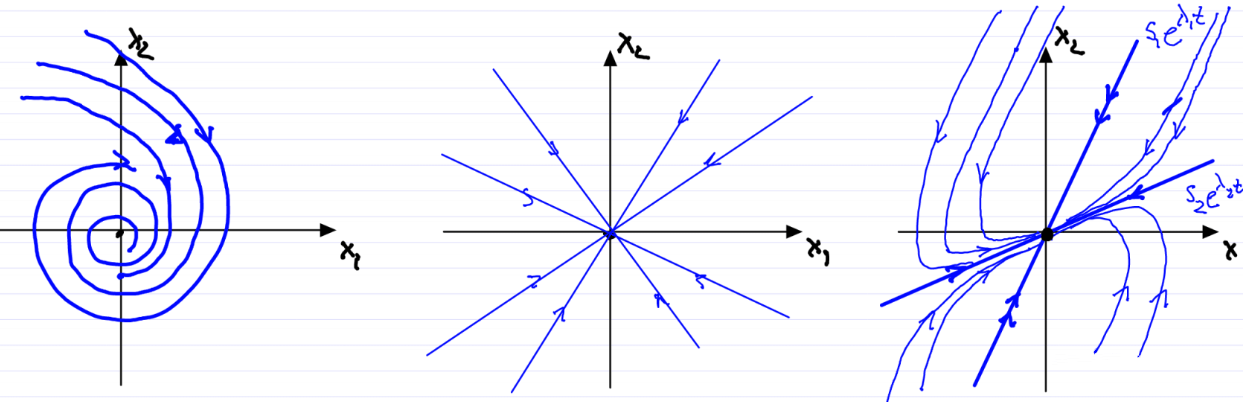
\includegraphics[width=0.9\textwidth]{figures/ch2/13topo_equiv.png}
		\caption{Three topologically equivalent 2-dimensional linear systems. Left: The stable spiral. Middle: The sink. Left: The stable node.}
		\label{fig:topo_equiv}
	\end{figure}

The stable spiral has the eigenvalues $\lambda _{1,2}= \alpha \pm i \beta $ for $\alpha <0$ and $\beta \neq 0$. The sink has the eigenvalues $\lambda_1=\lambda_2<0$. and The stable node has the eigenvalues $\lambda_1 < \lambda_2 < 0$. Note here that the number of eigenvalues $\lambda_i$ with $ \textrm{Re} \lambda_i <0$, $ \textrm{Re} \lambda _i=0$, and $ \textrm{Re} \lambda _i>0$ is the same is all three of these cases, namely for each system the real part of both eigenvalues are less than 0.	
\end{ex}

\begin{ex}[Topologically inequivalent linear systems for $n=2$]
	As a counter example, we now present three linear systems which are not topologically equivalent. The stable spiral (from before), the unstable spiral, and the saddle. The unstable spiral has the eigenvalues $\lambda _{1,2}= \alpha \pm i \beta $ for $\alpha > 0$ and $\beta \neq 0$ (note the different sign for $\alpha)$. The saddle has the eigenvalues $\lambda _1 < 0 < \lambda_2$. These systems are depicted in Fig \ref{fig:topo_inequiv}.
	\begin{figure}[h!]
		\centering
		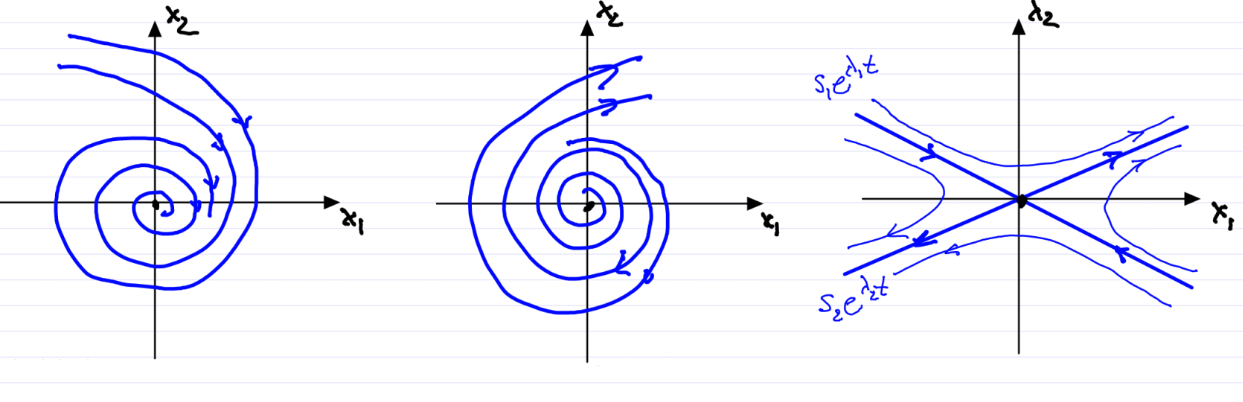
\includegraphics[width=0.9\textwidth]{figures/ch2/14topo_inequiv.png}
		\caption{Three 2-dimensional linear systems which are not topologically equivalent. Left: The stable spiral. Middle: The unstable spiral. Right: The saddle.}
		\label{fig:topo_inequiv}
	\end{figure}

	Note here that the eigenvalue configurations in terms of the number of $\lambda _i$ with real part less than $0$ are different in each case.
Building on the role of the eigenvalue configuration we noted in the previous examples, we introduce the concept of a hyperbolic fixed point.
\end{ex}
\begin{definition}[Hyperbolic fixed point]
	We call the fixed point  ${x} ={x_0} $ a \emph{hyperbolic fixed point} of \eqref{eq:unostar} if each of the eigenvalues $\lambda_i$ of its linearization \eqref{eq:dosstar} satisfy
	\begin{align}
		\boxed{ \textrm{Re} \lambda_i \neq 0.}
	\end{align}
	Geometrically the eigenvalue configuration of a hyperbolic fixed point is shown in Fig. \ref{fig:hyperbol_ex}.
	\begin{figure}[h!]
		\centering
		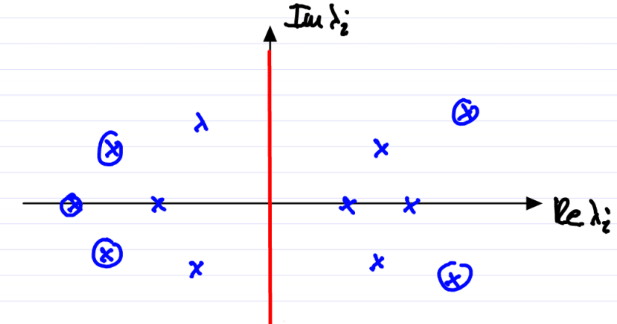
\includegraphics[width=0.6\textwidth]{figures/ch2/15hyperbol_ex}
		\caption{The eigenvalue configuration of a hyperbolic fixed point, i.e. no eigenvalues are on the imaginary axis (red).}
		\label{fig:hyperbol_ex}
	\end{figure}
\end{definition}
	
\begin{proposition}[]
	The linearized stability type of a hyperbolic fixed point is preserved under small perturbations to the nonlinear system.
\end{proposition}
Before proving this result, recall the Implicit Function Theorem (without proof).

\begin{theorem}[Implicit Function Theorem ($n+1$ dimensional case)]
	For a function $F:\mathbb{R}^{n+1} \to \mathbb{R}^{1}$ which is $C^1$, if  $F( {x_0} , y_0 ) = 0$ and the Jacobian $D_{{x} }F({x_0} , y_0 )$ is nonsingular (invertible), then there exists a nearby solution to $F({x} , y )=0 $, for ${x_y} = {x_0}  + \mathcal{O}(|y-y_0|)$. Further ${x_y} $ is as smooth in $y$ as $F({x} ,y)$.
\end{theorem}

\begin{proof}[Proof (Proposition)]
	Add a small perturbation to \eqref{eq:uno} i.e.
\begin{align}
	\dot{{x} } = f({x}) + \epsilon g({x} );\quad \|\epsilon \| \ll 1,\quad f({x} _0) =0.
\end{align}
Now we ask if the perturbed system has a fixed point ${x} _{\epsilon}$ near ${x} _0$? We frame this in terms of the implicit function theorem
\begin{align}
	F({x} ,\epsilon) = f({x} ) + \epsilon g({x} ) \stackrel{?}{=} 0;\quad F({x}_0, 0) = 0;\quad {x} \in \mathbb{R}^{n}, \quad F:\mathbb{R}^{n+1} \to \mathbb{R}^{1}.
\end{align}
We check that $D_{{x} }F({x_0} ,0) $ is nonsingular exactly when $Df({x_0)} $ is, this is fulfilled as we have no zero eigenvalues. The linearization at the perturbed fixed point takes the form
\begin{align}
	\dot{{y} } = D \left. \left[ f({x} ) + \epsilon g({x} ) \right]\right|_{{x} = {x_\epsilon} }{y} = \left[ Df({x_0}  + \mathcal{O}(\epsilon)) + \epsilon Dg({x_0} + \mathcal{O}(\epsilon)) \right] {y} 
		=\underbrace{ \left[ Df({x_0})+ \mathcal{O}(\epsilon) \right]}_{={A_{\epsilon}} }{y}.
\end{align}
In the last equality we used the Taylor expansion in $\epsilon$. We have that the roots of $\det({A_{\epsilon}}-\lambda {I} ) = 0 $ depend continuously on the parameter $\epsilon$. Therefore, the roots stay within an $\mathcal{O}(\epsilon)$ neighborhood of the eigenvalues of $Df({x_0} )$ (see Fig. \ref{fig:eps_ball_eigv}). Hence we have that the eigenvalue configuration is unchanged for small enough $\epsilon$.
\begin{figure}[h!]
	\centering
	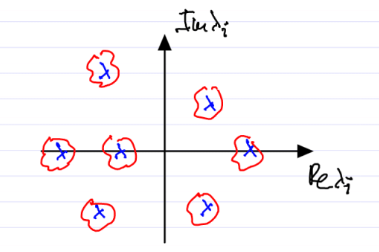
\includegraphics[width=0.5\textwidth]{figures/ch2/16eps_ball_eigv.png}
	\caption{The eigenvalue configuration the $\mathcal{O}(\epsilon)$ neighborhood (red) drawn around each eigenvalue (blue).}
	\label{fig:eps_ball_eigv}
\end{figure}
\end{proof}
\begin{remark}[]
	In the above proof, not only does the hyperbolicity of fixed points remain preserved, but also the stability type.
\end{remark}
Meanwhile, for nonhyperbolic fixed points, this is not the case, and the smallest perturbation may change their stability type. This is due to the fact, that no matter how small the scale of the perturbation ($\epsilon$) the $\mathcal{O}(\epsilon)$ ball around eigenvalues on the imaginary axis will always intersect with $\mathbb{C}\setminus \{  \textrm{Im}\lambda_i =0 \}$ (i.e. points which are not on the imaginary axis).

Now we would like to connect the preservation of stability type under nonlinear perturbation to analyzing the stability type of fixed points of nonlinear dynamical systems based on their linearization. 
\begin{theorem}[Hartman-Grobman]
	If the fixed point ${x_0} $ of the nonlinear system \eqref{eq:unostar} is hyperbolic, then the linearization \eqref{eq:dosstar} is topologically equivalent to the nonlinear system in a neighborhood of ${x_0} $. 

	\textbf{Consequence:} For hyperbolic fixed points, linearization predicts the correct stability type \underline{and} orbit geometry near ${x_0} $. 
\end{theorem}
Now we would like to apply this to the pendulum to systematically derive the stability type of its fixed points.
\begin{ex}[Stability analysis of the pendulum via Hartman-Grobman]
	Recall the transformed ODE for the pendulum
	\begin{align}
		\begin{dcases}
		\dot{x}_{1} = x_2 \\ \dot{x}_2 = -\sin(x_1)	
		\end{dcases}
		;\quad {x}  = 
		\begin{pmatrix}
			x_1 \\ x_2
		\end{pmatrix}
		.
	\end{align}
	We have two fixed points ${p} =(\pi ,0)$ and ${q} = (0,0)$. First we analyze the stability of the fixed point ${p} $. Start by linearizing at ${p} $ 
	\begin{align}
		\dot{{y} } = {Ay};\quad {A}  = Df({p} ) = 
		\begin{pmatrix}
			0 & 1 \\
			- \cos(x_1) & 0
		\end{pmatrix}_{{x} = {p} } =
		\begin{pmatrix}
			0 & 1 \\ 1 & 0
		\end{pmatrix}.
	\end{align}
	Now we have to check if ${p} $ is hyperbolic
	\begin{align}
		\det({A} - \lambda {I} ) = \lambda^2 -1 = 0 \implies \lambda_{1,2} = \pm 1;\ {s_1} =
		\begin{pmatrix}
			1 \\ 1
		\end{pmatrix}
		,\ {s_2} =
		\begin{pmatrix}
			-1 \\ 1
		\end{pmatrix}.
	\end{align}
	Neither of the eigenvalues lie on the imaginary axis, so $p$ is hyperbolic. This allows us to move between the nonlinear and linearized system for the stability analysis without compromising our results. We find the linearized dynamics to be
	\begin{align}
		{y} (t) = C_1 e^{t} {s_1}  + C_2 e^{-t}{s_2} = F^{t}{y_0} .
	\end{align}
	$F^{t}$ is the normalized fundamental matrix solution and ${y_0} $ is the initial condition. We can now fully describe the phase portrait of the linearization. The \emph{stable subspace} $E^{S}$ is $ \textrm{span} \{{s_2} \} = \{{y_0} :\ F^{t}{y_0} \xrightarrow{t \to \infty} 0 \} $. The unstable subspace $E^{U}$ is $ \textrm{span} \{{s_1}\} = \{{y_0} : \ F^{t}{y_0} \xrightarrow{t \to - \infty }0\} $. The phase portrait near the fixed point $p$ is illustrated in Fig. \ref{fig:pend_phase_p}
\begin{figure}[h!]
	\centering
	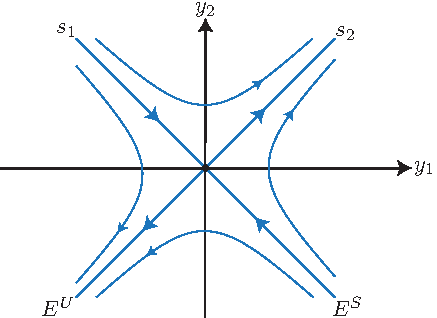
\includegraphics[width=0.4\textwidth]{figures/ch2/17pend_phase_p}
	\caption{The phase portrait of the linearized pendulum in a neighborhood around ${p} $.}
	\label{fig:pend_phase_p}
\end{figure}

The nonlinear phase portrait is topologically equivalent to the linear one. Further we can define the stable and unstable manifolds of ${p} $ for the nonlinear system. We designate $F^{t}(\cdot)$ to be the flow map for the nonlinear system after this point.
The \emph{stable manifold} of ${p} $ is 
\begin{align}
	\boxed{
	W^{S} = \{ {x_0} :\ F^{t}({x_0} ) \xrightarrow{t \to \infty}{p} \}.
}
\end{align}
and the \emph{unstable manifold} of ${p} $
\begin{align}
	\boxed{
	W^{U}=\{{x_0} :\ F^{t}({x_0} ) \xrightarrow{t \to - \infty}{p}\}.
}
\end{align}
Both of these are $C^{0}$ curves through ${p}$ and their existence follows from the Hartman-Grobman theorem. These manifolds are shown in the nonlinear phase portrait around ${p} $ in Fig. \ref{fig:nonlin_pend_phase_p}. 
\begin{figure}[h!]
	\centering
	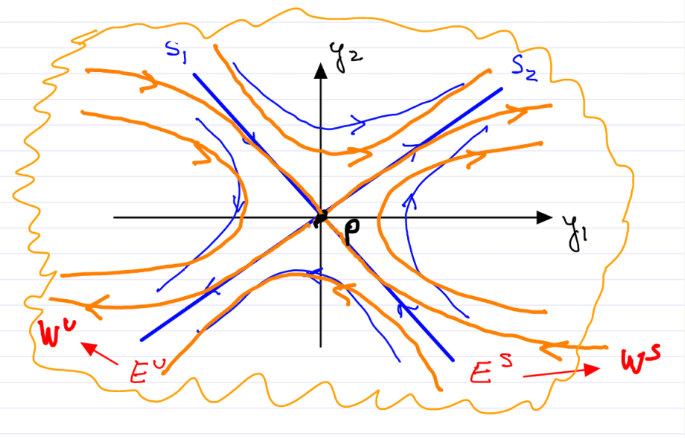
\includegraphics[width=0.6\textwidth]{figures/ch2/18nonlin_pend_phase_p.png}
	\caption{The phase portrait of the pendulum on a neighborhood around ${p} $ with the stable and unstable manifolds of the nonlinear system as well as the stable and unstable spaces of the linearization.}
	\label{fig:nonlin_pend_phase_p}
\end{figure}

\end{ex}

